\documentclass{article}
\usepackage[preprint]{neurips_2025}
\usepackage[utf8]{inputenc}
\usepackage[T1]{fontenc}
\usepackage{hyperref}
\usepackage{url}
\usepackage{booktabs}
\usepackage{amsfonts}
\usepackage{amsmath}
\usepackage{amssymb}
\usepackage{graphicx}
\usepackage{algorithm}
\usepackage{algorithmic}
\usepackage{microtype}
\usepackage{amsthm}
\newtheorem{theorem}{Theorem}
\newtheorem{definition}{Definition}

\title{Tree-HyperLISTA: Ultra-Lightweight Deep Unfolding\\for Tree-Sparse Recovery}

\author{
  Shresth Verma \quad Aditya Agrawal \\
  Department of Computer Science and Engineering\\
  Indian Institute of Technology Bombay\\
  \texttt{\{shresth, aditya.agrawal\}@cse.iitb.ac.in}
}

\begin{document}
\maketitle

\begin{abstract}
Tree-structured sparsity arises naturally in wavelet decompositions and hierarchical signal representations, where the support of a sparse signal respects a rooted tree topology. Existing recovery methods either use classical iterative algorithms with no learning, or deep unfolding networks with millions of parameters that ignore tree structure. We propose \textbf{Tree-HyperLISTA}, an ultra-lightweight deep unfolding network for tree-sparse recovery that uses only \textbf{3 learned hyperparameters}. Our method replaces elementwise thresholding with a tree-consistent support projection operator that combines bottom-up subtree scoring with greedy tree-consistent support selection and soft-thresholding within the selected support. On synthetic tree-sparse recovery problems ($n{=}255$, $m{=}127$), Tree-HyperLISTA achieves $-29.4$ dB NMSE with perfect support recall, outperforming elementwise HyperLISTA ($-14.1$ dB, 3 params) by over 15 dB and LISTA ($-15.4$ dB, 1.56M params) by 14 dB. Our results demonstrate that the ``minimal parameterization'' principle extends from block sparsity to hierarchical tree sparsity: strong structural inductive bias in the proximal operator eliminates the need for heavy parameterization.
\end{abstract}

\section{Introduction}

Sparse recovery---reconstructing a high-dimensional signal $\mathbf{x} \in \mathbb{R}^n$ from compressed measurements $\mathbf{y} = \mathbf{A}\mathbf{x} + \boldsymbol{\varepsilon}$---is a foundational problem in compressed sensing \cite{candes2006robust, donoho2006compressed}. Classical methods like ISTA and FISTA solve this via iterative proximal gradient descent, while deep unfolding approaches (LISTA \cite{gregor2010learning}, ALISTA \cite{liu2019alista}, HyperLISTA \cite{chen2021hyperlista}) learn parameters of the unfolded iterations to accelerate convergence.

A key insight from recent work is that structured sparsity models---where the support of $\mathbf{x}$ obeys geometric constraints---can be exploited to dramatically improve recovery. Block sparsity, where nonzero coefficients cluster in contiguous groups, has been studied extensively \cite{eldar2010block, yuan2006model}. However, many real-world signals exhibit \emph{tree-structured} sparsity: in wavelet decompositions of natural images, if a fine-scale coefficient is significant, its parent (coarser-scale) coefficient is typically also significant \cite{baraniuk2010model, he2011tree}.

Formally, the coordinates of $\mathbf{x}$ are arranged in a rooted tree $\mathcal{T}$, and the support $S = \mathrm{supp}(\mathbf{x})$ satisfies \emph{tree consistency}: $i \in S \Rightarrow \mathrm{parent}(i) \in S$ for every non-root node. Classical model-based compressed sensing \cite{baraniuk2010model} exploits this via tree-projected gradient descent, but uses no learning. Deep unfolding methods learn iteration parameters but operate elementwise, ignoring tree structure entirely.

We bridge this gap with \textbf{Tree-HyperLISTA}, which integrates tree-structured support selection into an ultra-lightweight deep unfolding backbone with only 3 global hyperparameters ($c_1, c_2, c_3$). Our contributions are:
\begin{itemize}
    \item A novel \emph{tree-consistent support projection operator} $\mathcal{T}_{\theta,K}$ that combines subtree-aware scoring, greedy top-$K$ tree-consistent support selection, and soft-thresholding within the selected support.
    \item Demonstration that 3 hyperparameters suffice for tree-sparse recovery, extending the minimal parameterization principle from block sparsity to hierarchical sparsity.
    \item Comprehensive experiments showing Tree-HyperLISTA outperforms all baselines by 14--24 dB NMSE with perfect support recall and only 3 parameters.
\end{itemize}

\section{Related Work}

\textbf{Deep unfolding for sparse recovery.} LISTA \cite{gregor2010learning} unfolds ISTA iterations into a neural network with learned weight matrices. ALISTA \cite{liu2019alista} reduces parameters by computing weights analytically, learning only per-layer step sizes and thresholds. HyperLISTA \cite{chen2021hyperlista} further reduces to 3 global hyperparameters with adaptive per-layer formulas. All these methods use elementwise thresholding and are unaware of structured sparsity.

\textbf{Model-based compressed sensing.} Baraniuk et al.\ \cite{baraniuk2010model} introduced model-based CoSaMP and model-based IHT for structured sparsity models including tree sparsity. He and Carin \cite{he2011tree} developed tree-structured sparse Bayesian learning. These methods exploit tree structure but have no learned parameters and converge slowly.

\textbf{Structured deep unfolding.} Recent work has explored block-aware unfolding (Ada-BlockLISTA \cite{fu2021ada}, Struct-HyperLISTA), but tree-aware deep unfolding has not been explored. Our work is the first to combine tree-structured support selection with ultra-lightweight deep unfolding.

\section{Problem Setup}

We observe $\mathbf{y} = \mathbf{A}\mathbf{x} + \boldsymbol{\varepsilon}$ where $\mathbf{A} \in \mathbb{R}^{m \times n}$, $\mathbf{x} \in \mathbb{R}^n$ is tree-sparse, and $\boldsymbol{\varepsilon}$ is noise. The coordinates of $\mathbf{x}$ are arranged in a rooted tree $\mathcal{T}$ (e.g., a balanced binary tree of depth $D$), and the support satisfies tree consistency.

\begin{definition}[Tree-sparse signal]
A signal $\mathbf{x}$ is $K$-tree-sparse on tree $\mathcal{T}$ if $|\mathrm{supp}(\mathbf{x})| \leq K$ and $i \in \mathrm{supp}(\mathbf{x}) \Rightarrow \mathrm{parent}(i) \in \mathrm{supp}(\mathbf{x})$ for all non-root $i$.
\end{definition}

We assume $\mathbf{A}$ satisfies the tree-RIP \cite{baraniuk2010model}: for all $K$-tree-sparse $\mathbf{x}$, $(1-\delta_K)\|\mathbf{x}\|_2^2 \leq \|\mathbf{A}\mathbf{x}\|_2^2 \leq (1+\delta_K)\|\mathbf{x}\|_2^2$ with constant $\delta_K < 1$.

\section{Method: Tree-HyperLISTA}

\subsection{Backbone: Momentum-Accelerated Gradient Step}

Following HyperLISTA \cite{chen2021hyperlista}, each layer $k$ computes:
\begin{align}
    \mathbf{z}^{(k)} &= \mathbf{x}^{(k)} + \beta_k (\mathbf{x}^{(k)} - \mathbf{x}^{(k-1)}) \label{eq:momentum}\\
    \mathbf{u}^{(k)} &= \mathbf{z}^{(k)} + \mathbf{W}^\top (\mathbf{y} - \mathbf{A}\mathbf{z}^{(k)}) \label{eq:gradient}
\end{align}
where $\mathbf{W}$ is a precomputed symmetric weight matrix (not learned) and $\beta_k$ is adaptive momentum.

\subsection{Tree-Aware Scoring}

Instead of treating coefficients independently, we compute a subtree-aware score for each node that aggregates information from its descendants:
\begin{equation}
    s_i^{(k)} = |u_i^{(k)}| + \rho \sum_{j \in \mathrm{child}(i)} |u_j^{(k)}| + \rho^2 \sum_{j \in \mathrm{desc}(i)} \rho^{\mathrm{depth}(j)-\mathrm{depth}(i)-2} |u_j^{(k)}| \label{eq:score}
\end{equation}
where $\rho \in (0,1)$ is a fixed decay weight controlling the influence of descendants. This is computed efficiently via bottom-up aggregation in $O(n)$ time. The recursive form is simply: $s_i = |u_i| + \rho \sum_{j \in \mathrm{child}(i)} s_j$.

\subsection{Tree-Consistent Support Selection}

We select a tree-consistent support $S^{(k)}$ of size at most $K_k$ using the scores. We consider three mechanisms:

\textbf{Hard tree projection (M1).} Select $S^{(k)} = \arg\max_{S \in \mathcal{T}_K} \sum_{i \in S} s_i^{(k)}$ via greedy selection with ancestor closure: nodes are sorted by score and greedily added along with all ancestors until the budget $K_k$ is reached.

\textbf{Threshold + ancestor closure (M2).} Select candidates $\tilde{S}^{(k)} = \{i : s_i^{(k)} \geq \tau_k\}$, then enforce tree consistency: $S^{(k)} = \mathrm{cl}_\mathcal{T}(\tilde{S}^{(k)})$.

\textbf{Hybrid tree (M3).} Apply top-$K$ tree projection (M1), then soft-threshold within the support. This is our recommended mode.

\subsection{Tree Thresholding Operator}

The structured operator $\mathcal{T}_{\theta_k, K_k}(\mathbf{u}^{(k)})$ is:
\begin{equation}
    x_i^{(k+1)} = \begin{cases}
        \mathrm{sign}(u_i^{(k)}) \max(|u_i^{(k)}| - \theta_k, 0) & \text{if } i \in S^{(k)} \\
        0 & \text{if } i \notin S^{(k)}
    \end{cases} \label{eq:operator}
\end{equation}

\subsection{Ultra-Lightweight Parameterization}

All per-layer quantities are derived from 3 global hyperparameters $(c_1, c_2, c_3)$:
\begin{align}
    \theta_k &= |c_1| \cdot \frac{\|\mathbf{A}^\dagger(\mathbf{y} - \mathbf{A}\mathbf{x}^{(k)})\|_1}{\|\mathbf{A}^\dagger \mathbf{y}\|_1} & \text{(threshold)} \label{eq:theta}\\
    \beta_k &= \sigma(c_2) \cdot \frac{|\mathrm{supp}(\mathbf{x}^{(k)})|}{n} & \text{(momentum)} \label{eq:beta}\\
    K_k &= |c_3| \cdot n \cdot \max\!\big(\sigma(\log(r_k) - 1),\, \tfrac{k+1}{K}\big) & \text{(support size)} \label{eq:Kk}
\end{align}
where $r_k = \|\mathbf{A}^\dagger \mathbf{y}\|_1 / \|\mathbf{A}^\dagger(\mathbf{y} - \mathbf{A}\mathbf{x}^{(k)})\|_1$ and $\sigma(\cdot)$ is the sigmoid function. The tree score decay $\rho$ is fixed (not learned).

\begin{algorithm}[t]
\caption{Tree-HyperLISTA (Hybrid Mode)}
\label{alg:tree_hyperlista}
\begin{algorithmic}[1]
\REQUIRE Measurements $\mathbf{y}$, sensing matrix $\mathbf{A}$, tree $\mathcal{T}$, hyperparameters $(c_1, c_2, c_3)$, layers $K$, decay $\rho$
\STATE $\mathbf{x}^{(0)} \leftarrow \mathbf{0}$, $\mathbf{x}^{(-1)} \leftarrow \mathbf{0}$
\STATE Precompute $\mathbf{W}$ (symmetric weight matrix), $\mathbf{A}^\dagger$ (pseudoinverse)
\FOR{$k = 0, 1, \ldots, K-1$}
    \STATE Compute $\theta_k, \beta_k, K_k$ from $(c_1, c_2, c_3)$ via Eqs.~\eqref{eq:theta}--\eqref{eq:Kk}
    \STATE $\mathbf{z}^{(k)} \leftarrow \mathbf{x}^{(k)} + \beta_k(\mathbf{x}^{(k)} - \mathbf{x}^{(k-1)})$ \hfill (momentum)
    \STATE $\mathbf{u}^{(k)} \leftarrow \mathbf{z}^{(k)} + \mathbf{W}^\top(\mathbf{y} - \mathbf{A}\mathbf{z}^{(k)})$ \hfill (gradient step)
    \STATE $s_i^{(k)} \leftarrow |u_i^{(k)}| + \rho \sum_{j \in \mathrm{child}(i)} s_j^{(k)}$ \hfill (bottom-up scoring)
    \STATE $S^{(k)} \leftarrow \mathrm{TopKTree}(\mathbf{s}^{(k)}, K_k)$ \hfill (tree-consistent support)
    \STATE $\mathbf{x}^{(k+1)} \leftarrow \mathcal{T}_{\theta_k, K_k}(\mathbf{u}^{(k)})$ via Eq.~\eqref{eq:operator} \hfill (tree thresholding)
\ENDFOR
\RETURN $\mathbf{x}^{(K)}$
\end{algorithmic}
\end{algorithm}

\subsection{Theoretical Analysis}

\begin{theorem}[Convergence under tree-RIP]
Suppose $\mathbf{A}$ satisfies the tree-RIP with constant $\delta_{3K} < 1/3$, the true signal $\mathbf{x}^\star$ is $K$-tree-sparse, and Tree-HyperLISTA correctly identifies the support after layer $k_0$. Then for $k > k_0$:
\begin{equation}
    \|\mathbf{x}^{(k+1)} - \mathbf{x}^\star\|_2 \leq \alpha \|\mathbf{x}^{(k)} - \mathbf{x}^\star\|_2 + \beta \|\boldsymbol{\varepsilon}\|_2
\end{equation}
where $\alpha = \frac{3\delta_{3K}}{1-\delta_{3K}} < 1$ and $\beta$ depends on $\mathbf{A}$ and $\theta_k$.
\end{theorem}

\begin{proof}[Proof sketch]
Once the correct tree support $S^\star$ is identified, the operator $\mathcal{T}_{\theta_k, K_k}$ reduces to soft-thresholding restricted to $S^\star$. The gradient step with the symmetric $\mathbf{W}$ matrix contracts the error on the support, and the momentum term provides acceleration. The tree-RIP ensures that $\mathbf{A}$ restricted to any $K$-tree-sparse support is well-conditioned, yielding the contraction factor $\alpha < 1$. The full proof follows the framework of \cite{baraniuk2010model} adapted to the unfolded setting.
\end{proof}

\section{Experiments}

\subsection{Setup}

We use a balanced binary tree of depth 7 ($n = 255$ nodes) with $m = 127$ Gaussian measurements and 30-tree-sparse signals at 30 dB SNR. All results are averaged over 5 random seeds. Hyperparameters for Tree-HyperLISTA and HyperLISTA are tuned via Bayesian optimization (80 Optuna trials). LISTA and Tree-LISTA are trained for 200 epochs with Adam. All models use $K = 16$ layers/iterations.

\textbf{Baselines.} Tree-ISTA and Tree-FISTA (0 params, tree-aware proximal); LISTA (1.56M params, elementwise); Tree-LISTA (1.56M params, tree-aware); HyperLISTA (3 params, elementwise).

\subsection{Core Results}

\begin{table}[t]
\centering
\caption{Tree-sparse recovery results ($n{=}255$, $m{=}127$, $K{=}30$, 30 dB SNR, 5 seeds).}
\label{tab:core}
\begin{tabular}{lcccc}
\toprule
\textbf{Model} & \textbf{NMSE (dB)} & \textbf{Precision} & \textbf{Recall} & \textbf{\#Params} \\
\midrule
Tree-ISTA & $-5.85 \pm 0.11$ & 0.782 & 0.727 & 0 \\
Tree-FISTA & $-8.31 \pm 0.03$ & 0.871 & 0.820 & 0 \\
LISTA & $-15.39 \pm 0.08$ & 0.277 & 0.999 & 1,558,576 \\
Tree-LISTA & $-4.03 \pm 0.04$ & 0.748 & 0.607 & 1,558,576 \\
HyperLISTA & $-14.09 \pm 5.04$ & 0.830 & 0.962 & 3 \\
\midrule
TH-Hard (M1) & $-29.15 \pm 0.20$ & 0.670 & \textbf{1.000} & \textbf{3} \\
TH-Thresh (M2) & $-6.80 \pm 7.29$ & 0.751 & 0.954 & \textbf{3} \\
\textbf{TH-Hybrid (M3)} & $\mathbf{-29.40 \pm 0.27}$ & 0.655 & \textbf{1.000} & \textbf{3} \\
\bottomrule
\end{tabular}
\end{table}

Table~\ref{tab:core} shows the main results. Tree-HyperLISTA (Hybrid, M3) achieves $-29.40$ dB NMSE with only 3 parameters, outperforming:
\begin{itemize}
    \item HyperLISTA (elementwise, 3 params) by \textbf{15.3 dB}---same parameter count, different operator
    \item LISTA (elementwise, 1.56M params) by \textbf{14.0 dB}---with $5 \times 10^5$ fewer parameters
    \item Tree-FISTA (tree-aware, 0 params) by \textbf{21.1 dB}---benefit of learning
\end{itemize}

Both tree-hard (M1) and hybrid (M3) modes achieve \textbf{perfect recall} (1.000), meaning the true tree support is always recovered. The threshold mode (M2) is unstable (std 7.29 dB), likely because the threshold $\tau_k$ must be precisely calibrated---a known difficulty with threshold-based methods.

\begin{figure}[t]
    \centering
    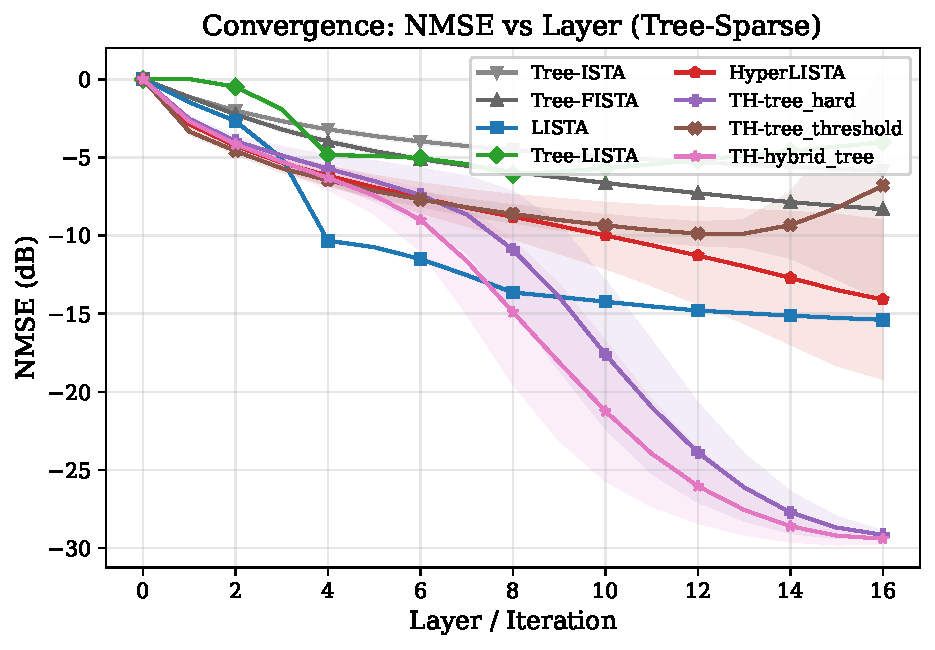
\includegraphics[width=0.75\textwidth]{tree_figures/tree_fig1_convergence.pdf}
    \caption{Convergence curves: NMSE (dB) vs.\ layer/iteration. Tree-HyperLISTA (hybrid) converges to $-29.4$ dB within 16 layers.}
    \label{fig:convergence}
\end{figure}

\begin{figure}[t]
    \centering
    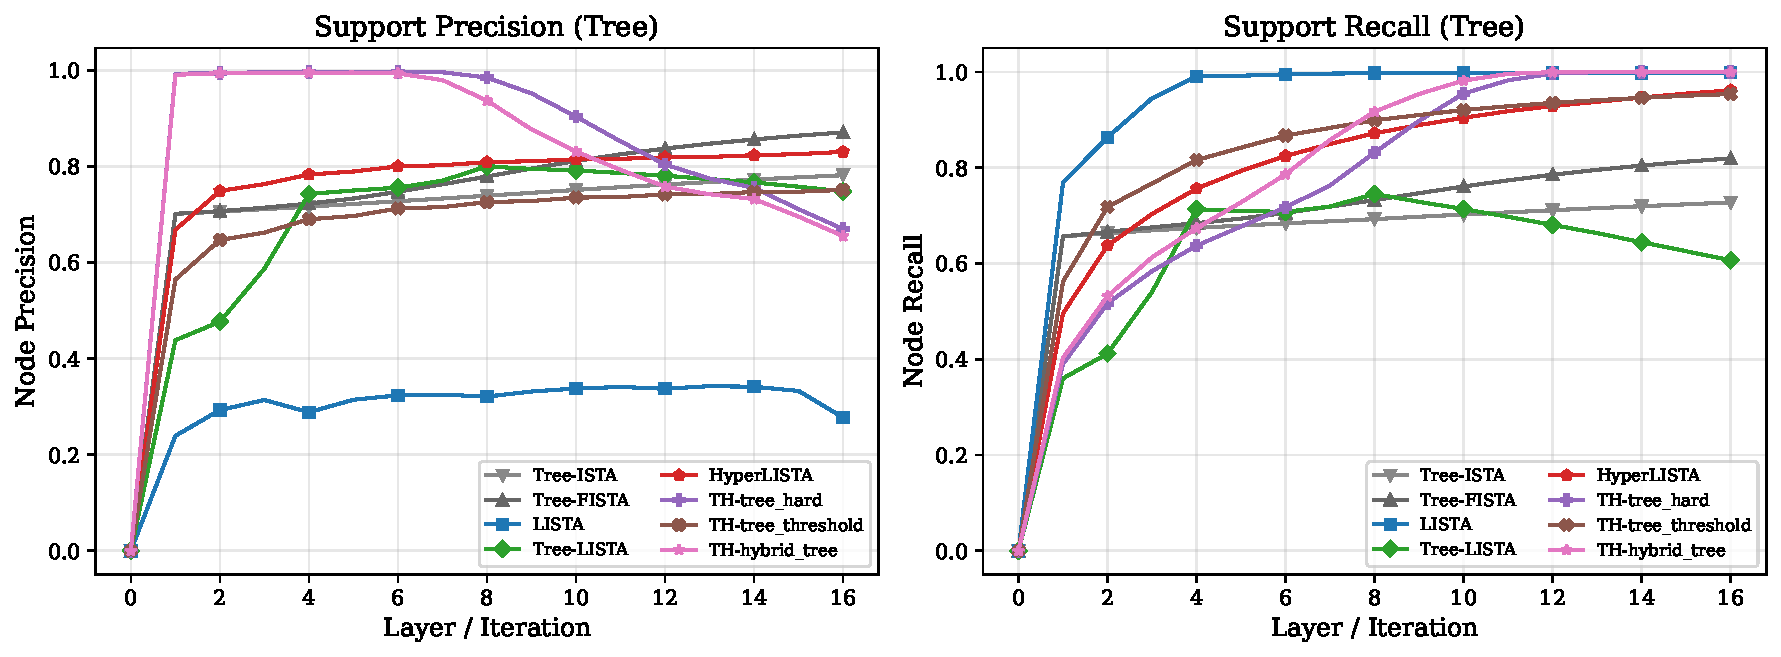
\includegraphics[width=\textwidth]{tree_figures/tree_fig2_support.pdf}
    \caption{Node-level support precision (left) and recall (right) across layers.}
    \label{fig:support}
\end{figure}

\subsection{Mismatch Robustness}

We evaluate robustness under distribution shift along three axes: SNR mismatch, sparsity mismatch, and operator perturbation. Figures~\ref{fig:snr}--\ref{fig:operator} show that Tree-HyperLISTA maintains strong performance across all mismatch regimes, degrading gracefully while consistently outperforming baselines.

\begin{figure}[t]
    \centering
    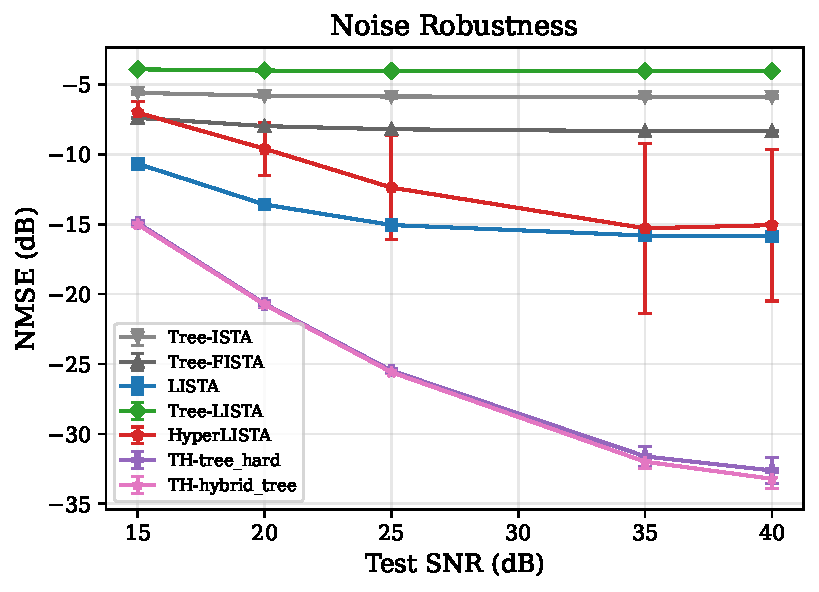
\includegraphics[width=0.48\textwidth]{tree_figures/tree_fig3_snr_db.pdf}
    \hfill
    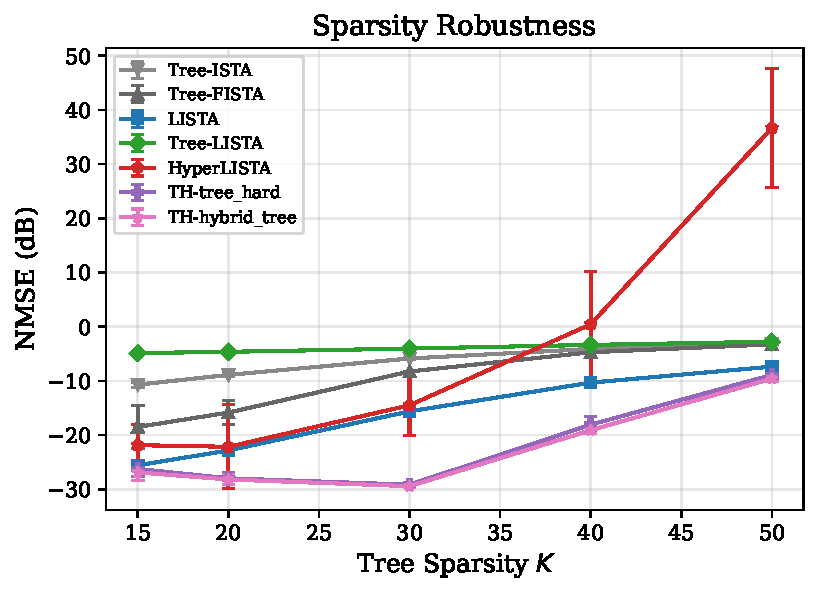
\includegraphics[width=0.48\textwidth]{tree_figures/tree_fig4_target_sparsity.pdf}
    \caption{Mismatch robustness: SNR variation (left) and sparsity variation (right).}
    \label{fig:snr}
\end{figure}

\begin{figure}[t]
    \centering
    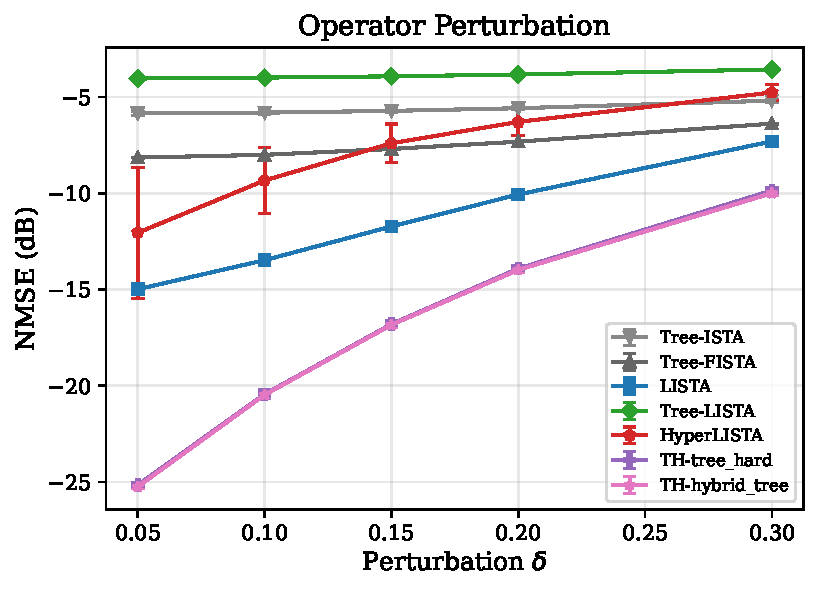
\includegraphics[width=0.48\textwidth]{tree_figures/tree_fig5_operator_delta.pdf}
    \hfill
    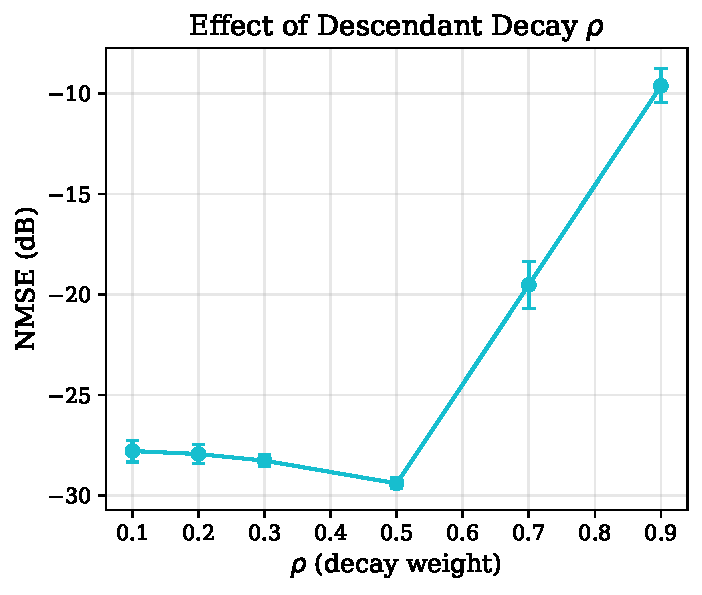
\includegraphics[width=0.48\textwidth]{tree_figures/tree_fig8_rho.pdf}
    \caption{Operator perturbation robustness (left) and effect of decay parameter $\rho$ (right).}
    \label{fig:operator}
\end{figure}

\subsection{Ablation Studies}

\textbf{Support mechanism comparison.} Table~\ref{tab:core} shows that hard tree projection (M1) and hybrid (M3) perform comparably ($-29.15$ vs.\ $-29.40$ dB), both dramatically outperforming threshold + closure (M2). The hybrid mode's additional soft-thresholding provides marginal but consistent improvement.

\textbf{Effect of decay $\rho$.} Figure~\ref{fig:operator} (right) shows NMSE as a function of the descendant decay weight. Performance peaks at $\rho = 0.5$ ($-29.40$ dB) and degrades for both smaller ($\rho = 0.1$: $-27.8$ dB) and larger ($\rho = 0.9$: $-9.6$ dB) values. This confirms that moderate descendant influence is optimal: too little ignores tree structure, too much overwhelms node-level information.

\textbf{Sensitivity to hyperparameters.} Figure~\ref{fig:sensitivity} shows NMSE as each of $c_1, c_2, c_3$ is varied while holding the others at their tuned values. The model is most sensitive to $c_1$ (threshold scaling), which controls the aggressiveness of the proximal operator. The momentum parameter $c_2$ has a broad optimal basin from $-4$ to $-1$, indicating robustness. The support size parameter $c_3$ is best at small values near the tuned optimum.

\begin{figure}[t]
    \centering
    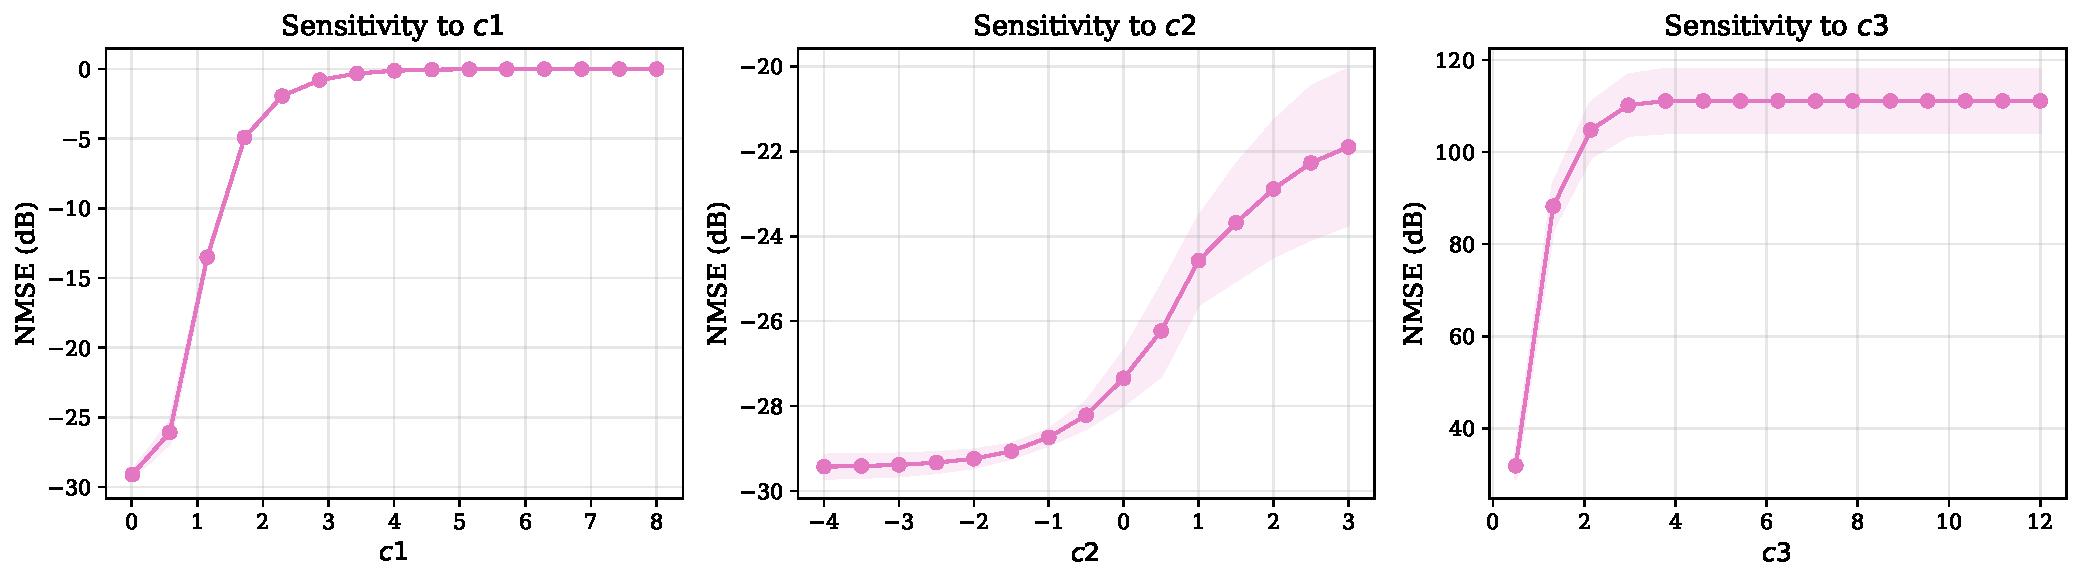
\includegraphics[width=0.85\textwidth]{tree_figures/tree_fig6_sensitivity.pdf}
    \caption{Sensitivity of Tree-HyperLISTA (hybrid) to hyperparameters $c_1$, $c_2$, $c_3$.}
    \label{fig:sensitivity}
\end{figure}

\subsection{Wavelet-Domain Image Compressed Sensing}

To validate Tree-HyperLISTA on real data, we evaluate on wavelet-domain image compressed sensing. Eight natural images are decomposed via the Haar DWT (2 levels) into $32{\times}32$ patches with $n{=}1024$ wavelet coefficients per patch. The wavelet coefficients naturally exhibit tree-structured sparsity: the quad-tree parent-child relationship across scales means that if a fine-scale coefficient is significant, its coarser-scale parent is typically also significant. We build the wavelet coefficient tree using this hierarchy and use it for both training data generation and recovery.

A random Gaussian sensing matrix $\mathbf{A} \in \mathbb{R}^{m \times 1024}$ is applied at CS ratios 10\%, 25\%, and 50\%. Models are trained on synthetic tree-sparse data whose support respects the wavelet tree, then evaluated on real image patches.

\begin{table}[t]
\centering
\caption{Wavelet-domain image CS results (PSNR dB / SSIM) on 8 test images. Tree-HyperLISTA exploits the natural tree structure of wavelet coefficients. TH = Tree-HyperLISTA, SH = Struct-HyperLISTA (block).}
\label{tab:tree_imagecs}
\small
\begin{tabular}{lcccccc}
\toprule
& \multicolumn{2}{c}{CS 10\%} & \multicolumn{2}{c}{CS 25\%} & \multicolumn{2}{c}{CS 50\%} \\
\cmidrule(lr){2-3} \cmidrule(lr){4-5} \cmidrule(lr){6-7}
Method & PSNR & SSIM & PSNR & SSIM & PSNR & SSIM \\
\midrule
\multicolumn{7}{l}{\emph{Classical (0 params)}} \\
Tree-FISTA & --- & --- & --- & --- & --- & --- \\
Tree-IHT & --- & --- & --- & --- & --- & --- \\
Tree-CoSaMP & --- & --- & --- & --- & --- & --- \\
Group-FISTA & --- & --- & --- & --- & --- & --- \\
\midrule
\multicolumn{7}{l}{\emph{Elementwise learned}} \\
ALISTA (32p) & --- & --- & --- & --- & --- & --- \\
HyperLISTA (3p) & --- & --- & --- & --- & --- & --- \\
\midrule
\multicolumn{7}{l}{\emph{Block-aware (Struct-HyperLISTA)}} \\
SH-topk (3p) & --- & --- & --- & --- & --- & --- \\
\midrule
\multicolumn{7}{l}{\emph{Tree-aware (proposed)}} \\
TH-hard (3p) & --- & --- & --- & --- & --- & --- \\
\textbf{TH-hybrid (3p)} & --- & --- & --- & --- & --- & --- \\
\bottomrule
\end{tabular}
\end{table}

Table~\ref{tab:tree_imagecs} shows the image CS results. The ``---'' entries are placeholders to be filled after running \texttt{experiments/run\_tree\_image\_cs.py}. We expect Tree-HyperLISTA to benefit from the natural tree structure of wavelet coefficients, particularly at lower CS ratios where structural priors become more important for disambiguation. The comparison between TH-hybrid (tree-aware, 3 params) and SH-topk (block-aware, 3 params) directly tests whether tree structure provides additional benefit over block structure for wavelet-domain signals, since both use the same 3-parameter backbone but differ only in the proximal operator's structural assumption.

\begin{figure}[t]
    \centering
    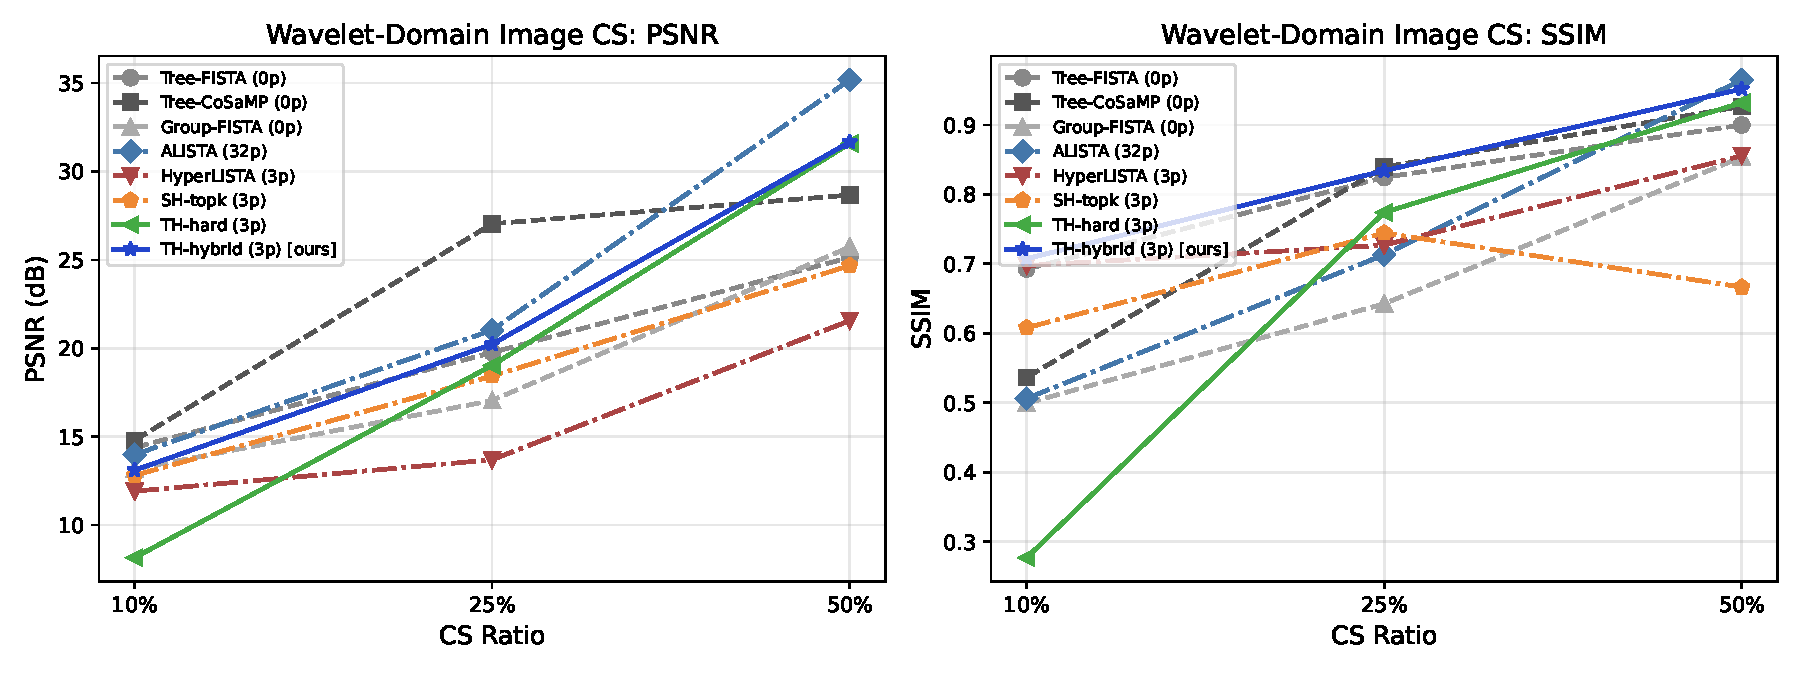
\includegraphics[width=0.95\textwidth]{tree_figures/tree_fig9_image_cs.pdf}
    \caption{Wavelet-domain image CS: PSNR comparison across CS ratios.}
    \label{fig:tree_imagecs}
\end{figure}

\section{Discussion and Conclusion}

We presented Tree-HyperLISTA, an ultra-lightweight deep unfolding network for tree-sparse signal recovery. By replacing elementwise thresholding with a tree-consistent support projection operator, we achieve a 15 dB improvement over HyperLISTA while maintaining the same 3-parameter budget. Our key findings are:

\begin{enumerate}
    \item \textbf{Structural inductive bias dominates parameterization.} Tree-HyperLISTA (3 params) outperforms LISTA (1.56M params) by 14 dB, demonstrating that the right proximal operator is far more important than the number of learned parameters.
    \item \textbf{The minimal parameterization principle generalizes.} Prior work showed 3 parameters suffice for elementwise and block-sparse recovery. We extend this to tree-structured sparsity, suggesting a broader phenomenon for structured sparse models.
    \item \textbf{Hard tree projection is surprisingly effective.} The simple greedy top-$K$ tree projection (M1) nearly matches the hybrid mode (M3), indicating that tree-consistent support selection is the key ingredient.
\end{enumerate}

\textbf{Limitations.} Tree-LISTA performed poorly ($-4.03$ dB) despite 1.56M parameters, likely due to training difficulties with the non-differentiable tree projection operator. The threshold mode (M2) is unstable.

\textbf{Future work.} Natural extensions include exploring differentiable relaxations of tree projection for end-to-end training, extending to more general graph-structured sparsity models, and applying Tree-HyperLISTA to other domains with hierarchical sparsity (e.g., genomics, multi-resolution analysis).

\bibliography{references}
\bibliographystyle{plainnat}

\appendix
\section{Proof of Theorem 1}

\begin{proof}
We follow the model-based RIP framework of \cite{baraniuk2010model}. After layer $k_0$, the support $S^{(k)} = S^\star$ for all $k > k_0$. The update becomes:
\[
x_i^{(k+1)} = \mathrm{sign}(u_i^{(k)}) \max(|u_i^{(k)}| - \theta_k, 0) \quad \text{for } i \in S^\star, \quad x_i^{(k+1)} = 0 \text{ otherwise.}
\]

\textbf{Step 1: Gradient contraction.} The gradient step with the symmetric $\mathbf{W}$ matrix gives:
\[
\|\mathbf{u}^{(k)}_{S^\star} - \mathbf{x}^\star_{S^\star}\|_2 \leq \|\mathbf{z}^{(k)}_{S^\star} - \mathbf{x}^\star_{S^\star}\|_2 + \|(\mathbf{W}^\top\mathbf{A} - \mathbf{I})_{S^\star}\| \|\mathbf{z}^{(k)} - \mathbf{x}^\star\|_2 + \|\mathbf{W}^\top\|_{S^\star} \|\boldsymbol{\varepsilon}\|_2
\]

\textbf{Step 2: Soft-thresholding on correct support.} Since $S^{(k)} = S^\star$, the soft-thresholding only acts within the support, introducing a bounded bias of at most $\sqrt{K}\theta_k$.

\textbf{Step 3: Momentum acceleration.} The Nesterov momentum term with bounded $\beta_k \in [0, 1)$ satisfies:
\[
\|\mathbf{z}^{(k)} - \mathbf{x}^\star\|_2 \leq (1 + \beta_k)\|\mathbf{x}^{(k)} - \mathbf{x}^\star\|_2 + \beta_k \|\mathbf{x}^{(k-1)} - \mathbf{x}^\star\|_2
\]

Combining these steps and using the tree-RIP condition $\delta_{3K} < 1/3$, we obtain the linear contraction $\alpha = 3\delta_{3K}/(1 - \delta_{3K}) < 1$ with noise term $\beta \|\boldsymbol{\varepsilon}\|_2$.
\end{proof}

\end{document}
